% !Mode:: "TeX:UTF-8"
\chapter{程序设计与实现}
\label{chapter-program}

以上三章分别介绍了 COSS 算法的整个流程以及各部分要解决的问题,并分别讨论了针对各问题的解决方案。本章将依据以上思路,用模拟程序分模块实现整个算法。
%本章介绍实现算法模拟的程序功能、各部分所用的数据结构及实现中所考虑的一些细节。

\section{程序结构及功能}
\label{sec-prgraom-structure}
% 总体功能,包括需要哪些输入信息,程序分成哪几块,各完成什么任务,最后输出什么信息等
% 不需要具体格式及数据结构
由于算法的功能是将带有周期性时间约束和数据依赖约束的任务在满足以上约束的条件下调度到一定拓扑结构的多核处理器(或多处理器结构)上去,因此程序的输入输出信息主要也就围绕这些内容来设置。

\subsection{输入信息}
%输入内容包括每个任务的属性、任务之间的数据依赖关系、多核之间的拓扑连接情况以及数据传输率。其中任务的自身属性包括在单个处理器上最坏情况下的执行时间(Worst Case Execution Time, WCET)、任务是否是自依赖的,对与周期任务$t_i$,还包括它的周期长度$T_i$、 首次释放时间$O_i$、 相对时间限$D_i$等情况。任务的数据依赖关系$\textnormal{Dep}_{ij}=\{i,j,p_{ij},c_{ij},D_{ij}\}$ 是指两个任务$t_i$ 与$t_j$之间,$t_i$ 每执行一次,将向$t_j$ 发送$p_{ij}$ 个数据,而$t_j$ 每执行一次,将消耗从$t_i$ 发来的$c_{ij}$ 个数据。此外,$\textnormal{Dep}_{ij}$还包括初始状态下$t_i$ 与$t_j$ 之间已存在的可由$t_j$直接使用的数据量$D_{ij}$。最后,为得到较理想的调度结果,还需输入周期倍数参数$J$,表示程序在寻找可行调度时需在大周期中包含多少个最小周期。

程序的输入信息主要包括任务属性以及目标平台属性两方面内容。

\begin{enumerate}
  \item 任务属性
    \begin{itemize}
      \item 对每个任务 $t_i$,最坏情况下的执行时间$C_i$(Worst Case Execution Time, WCET)
      \item 任务是否是自依赖的(即是否必须串行执行)
      \item 对于周期性任务 $t_i$,包括周期长度$T_i$、 首次释放时间$O_i$、 相对时间限$D_i$ 等。
      \item 任务之间的依赖关系 $\textnormal{Dep}_{ij}=\{i,j,p_{ij},c_{ij},D_{ij}\}$。 指的是两个任务$t_i$ 与$t_j$之间,$t_i$ 每执行一次,将向$t_j$ 发送$p_{ij}$ 个数据,而$t_j$每执行一次,将消耗从$t_i$ 发来的$c_{ij}$ 个数据,以及初始状态下$t_i$ 与$t_j$ 之间已存在的可由$t_j$直接使用的数据量$D_{ij}$。
    \end{itemize}
  \item 目标平台属性
    \begin{itemize}
      \item 处理器的核数 M
      \item 两两核之间的连接情况,即连接矩阵
      \item 核间数据传输速率 s
    \end{itemize}
\end{enumerate}

此外,为得到更好的调度结果,有时还需要指定在一个调度大周期中包含多少个最小调度周期,即周期倍数 $J$。


\subsection{输出信息}

根据以上输入信息,如果程序针对目标平台能够找到可行调度,程序将输出两类调度列表:
\begin{enumerate}
  \item 针对每一个处理器核心生成任务调度表
  \item 针对每一条核间链路生成其上的消息调度表
\end{enumerate}

为补充输出信息的完整性,每个任务在周期内的多次执行在各个核上的空间与时间分布情况也将输出。此外,为反映算法过程,程序各步的中间结果信息也将会输出。

\subsection{程序结构}
从结构上来说,算法的模拟程序与 COSS 算法的整体流程相一致,主要分为数据输入、构建GSDF 图、从GSDF 构建DAG 最终由 DAG 生成调度表等几个模块。程序总的数据流程如图 \ref{PROG-fig-flow} 所示。

\begin{figure}[!hbt]
  \centering
  % Requires \usepackage{graphicx}
  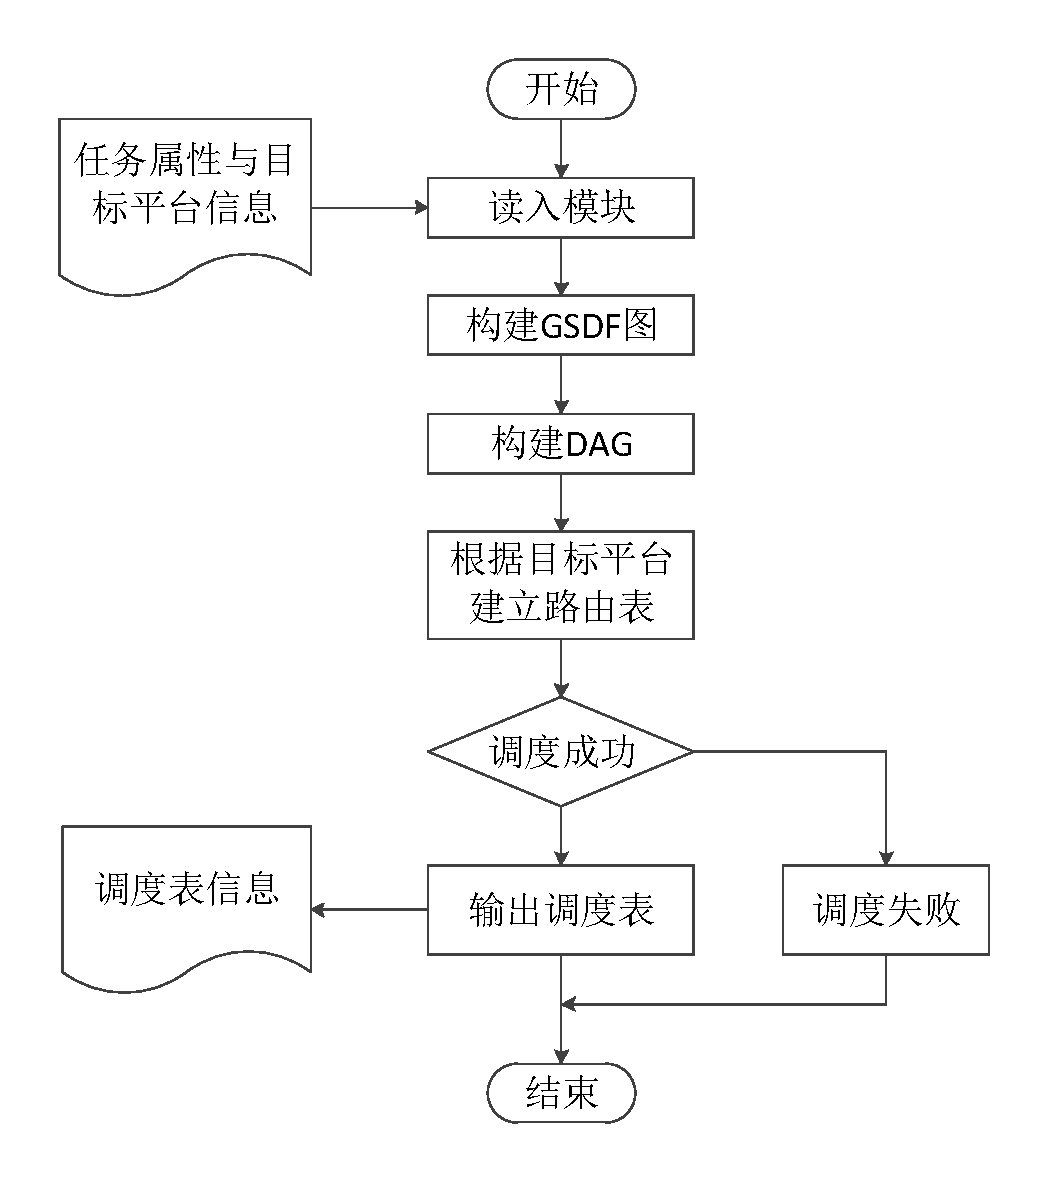
\includegraphics[height=55ex]{figure/PROG-flow.pdf}\\
  \caption{算法程序流程图}\label{PROG-fig-flow}
\end{figure}

根据以上流程,程序的功能模块划分如图\ref{PROG-fig-module}所示,各模块对应文件如表\ref{program-tab-file}所示。

\begin{figure}[!hbt]
  \centering
  % Requires \usepackage{graphicx}
  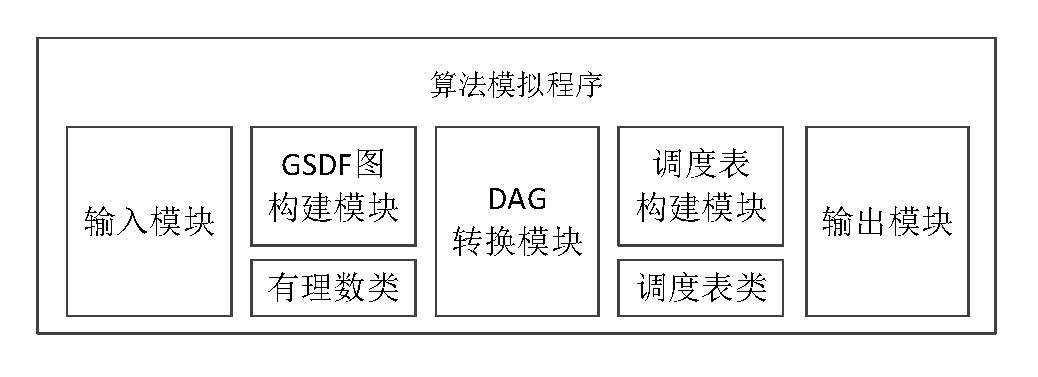
\includegraphics[height=20ex]{figure/PROG-module.pdf}\\
  \caption{模拟程序功能模块划分}\label{PROG-fig-module}
\end{figure}

{\renewcommand{\arraystretch}{1.5}
\begin{table}
  \centering
  \caption{程序文件描述}
  \label{program-tab-file}
  \begin{tabular}{|l|l|}
    \hline
    % after \\: \hline or \cline{col1-col2} \cline{col3-col4} ...
    Config.h & 设定任务数上限、调整浮点数计算精度等程序设置 \\
    input.cpp & 输入模块,读取输入数据并储存 \\
    Rational.h & 提供用于分数计算的类,解矩阵方程时用到 \\
    SDF.cpp & 从时间约束和数据约束构建 GSDF 图,并求解最小周期 \\
    DAG.cpp & ICS 算法从 GSDF 构建 DAG \\
    ScheduleList.h & 提供调度表类,方便对调度表的添加任务、查找空闲时间等操作 \\
    StaticSchedule.cpp & 消息路由、MDLS 算法从 DAG 求得调度表 \\
    main.cpp & 主程序\\
    \hline
  \end{tabular}
\end{table}
}

\section{详细设计}
每一模块的功能实现部分主要按照三、四、五章中的具体算法来完成。本节介绍在实现过程中存储结构的选择以及遇到的一些细节优化问题。

\subsection{数据输入}
\label{sec-data-structure}

每个任务的时间属性用一个 Task 结构体来表示,任务间通信关系用一个 Arc 结构体来表示,如表 \ref{program-tab-code-task} 所示。

{\renewcommand{\arraystretch}{1.5}
\begin{table}
  \caption{任务属性的结构体}
  \label{program-tab-code-task}
  \begin{lstlisting}[
      language={C},
      caption={}
      %label={program-code-task},
  ]
    // 时间约束
    struct Task
    {
        int wcet;        // 最坏运行时间
        int T;           // 周期
        int offset;      // 首次释放偏移
        int deadline;    // 时间限
        int selfdelay;   // 任务是否是自依赖的
                         // >0: 任务自依赖,运行时间需要数据通信
                         // =0: 任务自依赖,需要串行调度,但无数据通信
                         // <0: 任务不是自依赖,可以并行调度
    };

    // 数据依赖约束
    struct Arc
    {
        int src;         // 源任务结点
        int produce;     // 每次执行产生的数据
        int snk;         // 目标任务结点
        int consume;     // 每次执行消耗的数据
        int delay;       // 初始时弧上的 Delay
    };
  \end{lstlisting}
\end{table}
}

输入任务的信息和通信关系分别用一个数组 tasks 和 arcs 表示。

\subsection{GSDF图数据结构}

按第\ref{chapter-SDF}章所述算法可构建 GSDF 图。常用的图存储模式有邻接矩阵与邻接表,一般邻接矩阵适合于边稠密的图,而 GSDF 图中边数主要与任务间的数据依赖关系数有关,全部任务两两之间都有数据依赖的情况较少见,因此程序选择邻接表存储方式,空间占用与边的多少相关。GSDF 图的存储结构如图 \ref{PROG-fig-GSDF-structure} 所示。
为了方便遍历,我们不仅将某结点的出弧存储在此结点对应链表中,该结点的入弧同样也存储进来,这样从一个结点出发即可访问所有和它有数据依赖关系的全部结点,为求解拓扑矩阵提供方便。此外,在存储结构中将 GSDF 的反向弧也保存在邻接表中,这样,在修改某条弧上的缓冲区数值时,对应反向弧也方便一起修改,免去查找过程。

\begin{figure}[!hbt]
  \centering
  % Requires \usepackage{graphicx}
  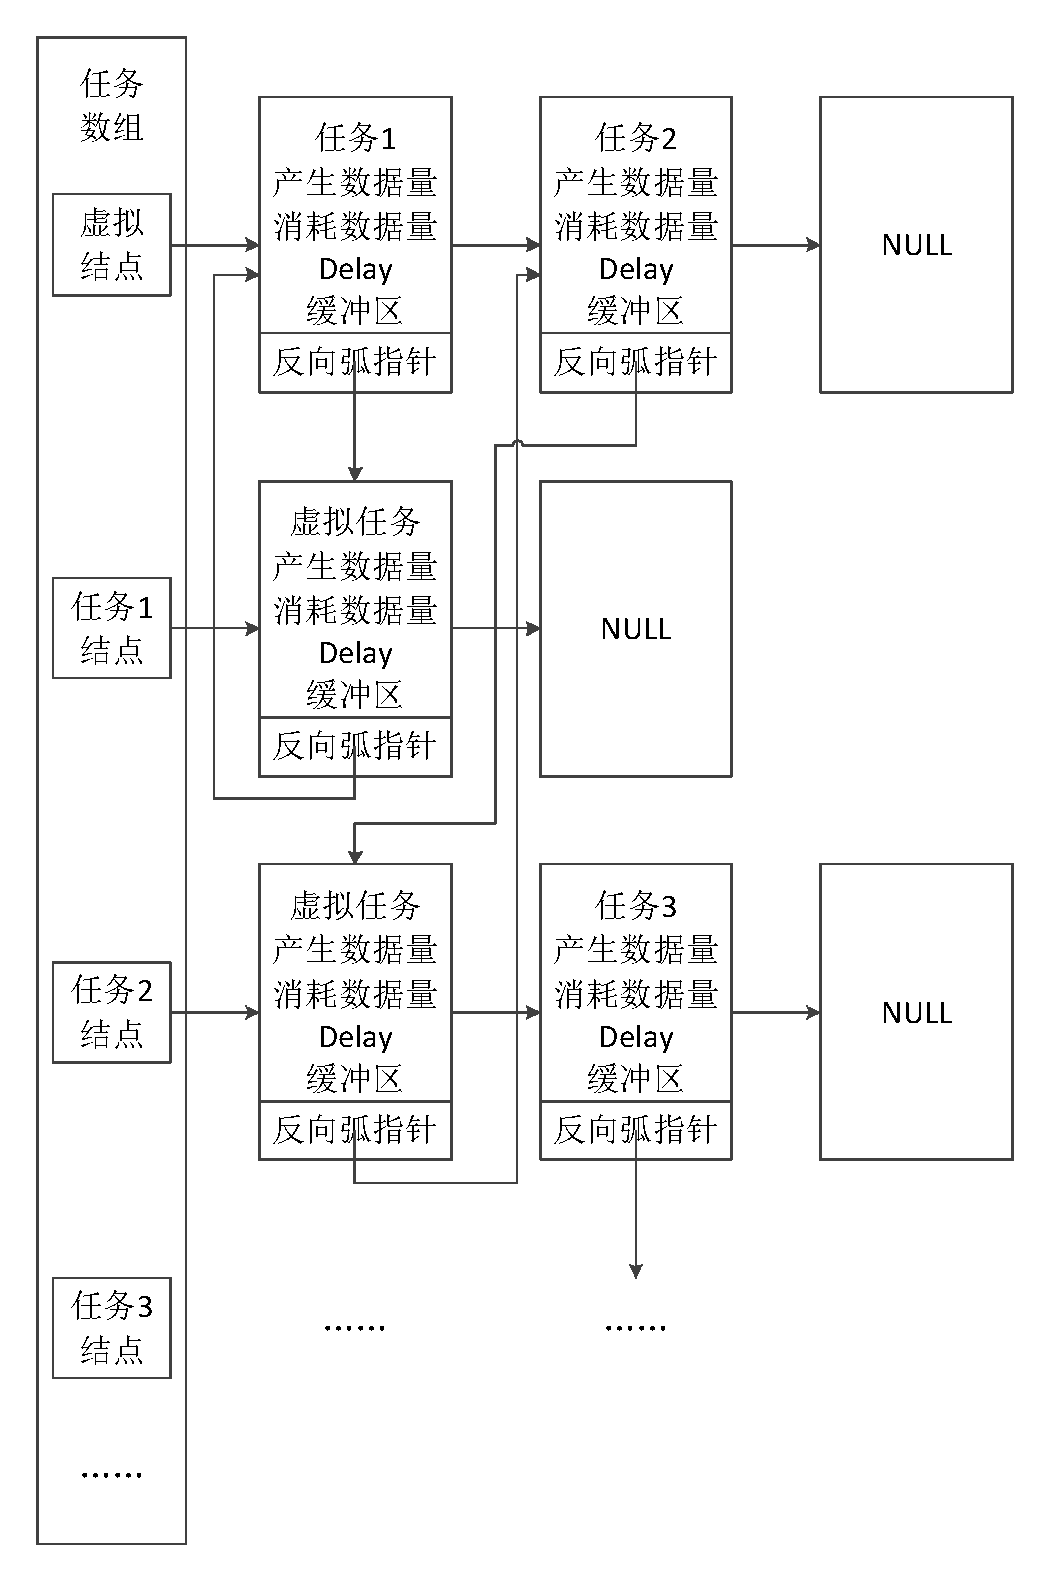
\includegraphics[height=63ex]{figure/PROG-fig-GSDF-structure.pdf}\\
  \caption{GSDF 数据结构图}\label{PROG-fig-GSDF-structure}
\end{figure}


%边的数据结构如代码 \ref{program-code-GSDF} 所述
%
%\begin{lstlisting}[
%    language={C},
%    caption={GSDF 的数据结构},
%    label={program-code-GSDF},
%]
%struct AdjNode
%{
%    int toTaskIdx;
%    int produce;    // < 0 on revarcs in sdf
%    int consume;    // < 0 on revarcs in sdf
%    int delay;      // always 0 on revarcs in sdf
%    int buffer;     // always 0 on revarcs in sdf
%    AdjNode *revarc;
%};
%
%list<AdjNode> sdf[MAXTASKNUM];    // sdf[0] is the virtual node,
%                                  // sdf[1]~sdf[N] are task nodes.
%\end{lstlisting}

在求解拓扑矩阵时,考虑到矩阵的特殊性质:每行仅有两个非零值,且一正一负。由以上特性可知向量解中两两分量间的比例关系,直接在 GSDF 图中采用一次深度优先遍历即可求得所有分量间的比例关系,取其最小公倍数,即容易得出拓扑矩阵的最小整数解向量,大幅降低了解方程的复杂度。为了求解拓扑矩阵,本模块还对有理数的运算做了封装,用于对分数运算的精确处理,以及最后求解分数的公倍数提供方便。

%\subsection{从GSDF到DAG}
% 矩阵解法
% 等等
%\emph{TODO: 矩阵解法}


%\emph{TODO: 结点间数据传输的处理}
%关于上一章提到的处理周期内与周期间数据传输的问题,由于细节处理方面判断分支很多,代码量较大,请具体参阅程序源码对应部分。

\subsection{目标平台的下一跳矩阵}
% 所有点对间最短路
%\emph{TODO: 所有点对间无权图最短路径}
按上一章所述,处理器间消息传递的路由选择按最少跳数进行。模拟程序为输入方便,仅输入了目标处理器平台的连接矩阵,因此程序在确定消息路径之前需要计算核之间的无权最短路径,并得到目标平台的下一跳矩阵。
模拟程序中由处理器之间连接关系的邻接矩阵直接构建所有核之间的下一跳矩阵,采用层级广度优先遍历的顺序,在找到最短消息路径的同时,也将下一跳信息储存下来,形成下一跳矩阵。


%在进行 DLS 算法之前,首先求出目标平台所有核间的最短通路,并求出指向最短通路的下一跳矩阵。
% 给出求下一跳矩阵的算法描述

\subsection{用MDLS方法构建静态调度表}

在调度表构建模块中,为方便对调度表的操作,模拟程序设计了 ScheduleList 类,将与调度表的有关操作封装起来,专用来处理与调度表相关的任务。其类声明如表 \ref{program-code-SchList} 所示。

{\renewcommand{\arraystretch}{1.5}
\begin{table}
  \caption{调度表类}
  \label{program-code-SchList}
    \begin{lstlisting}[
        language={C},
        caption={}
    ]
    template<class DataType>
    class ScheduleList
    {
    public:
        double lastSlot() const;
        double findSlot(double stTime, double span) const;
        bool insertWork(double time, double span, const DataType &data);

        // 保存当前状态
        void save();
        // 回退到上一次保存的状态
        void drawback();

        void print(FILE *fp, char *preStr) const;
    };
    \end{lstlisting}
  \end{table}
}

在实现 MDLS 算法中,需要频繁操作对应各个处理器和链路上的调度表,因此有必要将其独立出来作为一个类专门处理关于调度表的各项操作,例如添加一个新任务安排,查找满足一定条件的时间空隙等等。特别的,为了处理 MDLS 中因尝试调度计算最早开始时间而产生的回溯情况,在此类中添加保存状态和恢复保存的状态接口,为程序编排和代码逻辑清晰度都带来很大好处。ScheduleList 类的主要接口功能如表 \ref{program-tab-SchList-mem} 所示。其中 drawback() 在恢复时实际使用 swap 方法,只交换指针不交换调度表内容即可将调度表状态还原,减少了数据复制的开销。

{\renewcommand{\arraystretch}{1.5}
\begin{table}
  \centering
  \caption{调度表类的接口功能说明}
  \label{program-tab-SchList-mem}
  \begin{tabular}{l|l}
    \hline
    lastSlot() & 返回最后一个空闲时间段的起始时间 \\
    findSlot() & 从给定的时间开始向后,找到一个大于给定值的空闲时间段,返回开始时间 \\
    insertWork() & 想调度表中添加新的任务安排\\
    \hline
    save() & 为方便 MDLS 调度中储存临时状态以便调度不成功时回溯,此函数可保存调\\
           & 度表当前状态 \\
    drawback() & 将调度表恢复到上一次保存的状态。\\
    \hline
    print() & 打印调度表\\
    \hline
  \end{tabular}
\end{table}
}


\section{本章小结}

本章设计并实现了COSS算法的模拟程序。文中首先根据算法流程对模拟程序的功能模块做了划分,并设计了程序的输入输出文件格式。其次,针对程序实现过程中相关信息存储时数据结构的选择等问题提出了代码优化方案,并给出了实现方式。最后,本章对调度表构建模块中对调度表所需的一些具体操作进行了封装,并提出了采用 swap 方式优化状态保存及返回状态两个操作。

